\documentclass[aspectratio=169,10pt]{beamer}

% Theme and styling (same look as the earlier decks)
\usetheme{Madrid}
\usecolortheme{whale}
\setbeamertemplate{navigation symbols}{}
\setbeamertemplate{caption}[numbered]
\setbeamerfont{caption}{size=\footnotesize}

\usepackage{amsmath,amssymb,amsfonts}
\usepackage{booktabs}
\usepackage{tabularx}
\usepackage{graphicx}
\usepackage{hyperref}
\usepackage{xcolor}
\usepackage{colortbl}

\graphicspath{{figures/}{figures/volatility/}}

\definecolor{primaryblue}{RGB}{20, 50, 110}
\definecolor{accentblue}{RGB}{41, 128, 185}
\definecolor{darkgray}{RGB}{50, 50, 50}
\definecolor{lightgray}{RGB}{246, 248, 250}
\definecolor{mathred}{RGB}{192, 57, 43}
\definecolor{mathgreen}{RGB}{39, 174, 96}

\setbeamercolor{palette primary}{bg=primaryblue,fg=white}
\setbeamercolor{palette secondary}{bg=accentblue,fg=white}
\setbeamercolor{structure}{fg=primaryblue}
\setbeamercolor{title}{bg=primaryblue,fg=white}
\setbeamercolor{block title}{bg=primaryblue!12,fg=primaryblue}
\setbeamercolor{block body}{bg=lightgray,fg=darkgray}
\setbeamercolor{block title alerted}{bg=mathred!15,fg=mathred}
\setbeamercolor{block body alerted}{bg=lightgray,fg=darkgray}
\setbeamercolor{block title example}{bg=mathgreen!15,fg=mathgreen!70!black}
\setbeamercolor{block body example}{bg=lightgray,fg=darkgray}

\newcommand{\takeaway}[1]{\vspace{2pt}\begin{exampleblock}{}\small #1\end{exampleblock}}
\newcommand{\yes}{\textcolor{mathgreen!70!black}{\textbf{yes}}}
\newcommand{\no}{\textcolor{mathred}{\textbf{no}}}

\title[\textbf{Nonlinear Analysis of BTC}]{\Large \textbf{Is Bitcoin Chaotic?}\\\large Nonlinear and Chaos Analysis of BTC Returns and Volatility}
\subtitle{Phase-space reconstruction, chaos tests and surrogate data}
\author[\textbf{Anuj Kothari}]{Anuj Kothari}
\date{\today}

\begin{document}

\begin{frame}
    \titlepage
\end{frame}

\begin{frame}{Outline}
    \tableofcontents
\end{frame}

% ==============================================================================
\section{Question and Method}

\begin{frame}{1. The Question}
    \begin{columns}[T]
        \begin{column}{0.5\textwidth}
            \begin{block}{Two questions, kept separate}
                \small
                \begin{enumerate}
                    \item \textbf{Nonlinearity:} is there dependence that a linear Gaussian process cannot produce?
                    \item \textbf{Deterministic chaos:} is that nonlinearity generated by a low-dimensional deterministic system, rather than by randomness?
                \end{enumerate}
            \end{block}
            \small
            A series can be clearly \textbf{nonlinear} and still be \textbf{random}: volatility clustering (GARCH) is the standard example.
        \end{column}
        \begin{column}{0.46\textwidth}
            \begin{alertblock}{Why care}
                \small
                Chaos is deterministic, so it is \textbf{predictable over short horizons}. Randomness is not.
                Finding chaos in BTC would mean nonlinear forecasting models should work.
            \end{alertblock}
            \begin{block}{Ground rules}
                \small
                No plot and no single test may decide ``chaos''. Every statistic is compared with \textbf{surrogate} series that are random by construction.
            \end{block}
        \end{column}
    \end{columns}
\end{frame}

\begin{frame}{2. Data and the Four Series}
    \centering
    \small
    BTC daily close (Binance), 2017-08-17 to 2026-09-02, $n \approx 3300$ days. The data file is only read.

    \vspace{8pt}
    \begin{tabular}{lll}
        \toprule
        Series & Definition & Measures \\
        \midrule
        returns & $r_t = \ln P_t - \ln P_{t-1}$ & direction and size of the move \\
        absolute returns & $\lvert r_t \rvert$ & daily volatility \\
        squared returns & $r_t^2$ & daily variance \\
        20-day realised volatility & $RV_t = \sqrt{\tfrac{1}{20}\sum_{i=0}^{19} r_{t-i}^2}$ & smoothed volatility \\
        \bottomrule
    \end{tabular}

    \vspace{8pt}
    \raggedright
    \begin{itemize}\small
        \item Part A: returns only (notebook \texttt{chaos\_classification}).
        \item Part B: all four series side by side (notebook \texttt{volatility\_chaos}).
    \end{itemize}
\end{frame}

\begin{frame}{3. Toolkit in Plain Words}
    \centering
    \footnotesize
    \begin{tabularx}{\textwidth}{lX}
        \toprule
        Tool & What it asks \\
        \midrule
        Return map, phase space & Do the points form a thin, folded shape (attractor) or a blob (noise)? \\
        Recurrence plot & When the series revisits a state, does it then follow the same path (long diagonal lines)? \\
        Average Mutual Information & After how many days ($\tau$) does today stop telling us much about the future? \\
        False Nearest Neighbours & How many dimensions ($m$) are needed to unfold the dynamics? Noise never unfolds. \\
        Largest Lyapunov exponent & Do nearly identical states drift apart exponentially? \\
        Correlation dimension $D_2$ & Is the data on a low-dimensional object ($D_2$ stops growing with $m$)? \\
        0--1 test & Regular ($K\approx0$) or irregular ($K\approx1$)? Noise also gives $K\approx1$. \\
        Time-reversal asymmetry & Does the series look different when played backwards? \\
        S-map gain, prediction skill & Does a local nonlinear forecast beat a linear one? \\
        \bottomrule
    \end{tabularx}
\end{frame}

\begin{frame}{4. Surrogate Data and the Decision Rule}
    \begin{columns}[T]
        \begin{column}{0.52\textwidth}
            \centering
            \footnotesize
            \begin{tabular}{lll}
                \toprule
                Surrogate & Keeps & Rejecting it means \\
                \midrule
                IAAFT & distribution, spectrum & nonlinearity \\
                GARCH(1,1)-$t$ & fat tails, vol clustering & beyond a stochastic \\
                & & volatility model \\
                \bottomrule
            \end{tabular}
            \vspace{6pt}
            \raggedright
            \begin{itemize}\footnotesize
                \item GARCH surrogates are simulated returns put through the \textbf{same} transformation as the data.
                \item 99 (Part A) and 999 (Part B) surrogates per family; Benjamini--Hochberg FDR over the 48 tests of Part B.
            \end{itemize}
        \end{column}
        \begin{column}{0.45\textwidth}
            \begin{block}{Classification rule (fixed in advance)}
                \footnotesize
                \textbf{Periodic / quasi-periodic:} $K<0.2$ and $D_2$ saturates.\\[2pt]
                \textbf{Potentially chaotic:} $K>0.8$, $D_2$ saturates, and $\ge2$ statistics differ from \textbf{both} IAAFT and GARCH.\\[2pt]
                \textbf{Random/Stochastic:} $K>0.8$ and nothing differs from GARCH.\\[2pt]
                \textbf{Inconclusive:} anything else.
            \end{block}
        \end{column}
    \end{columns}
    \takeaway{A positive Lyapunov exponent alone never counts: random series give one too.}
\end{frame}

% ==============================================================================
\section{Part A: BTC Returns}

\begin{frame}{5. Returns and the Return Map}
    \centering
    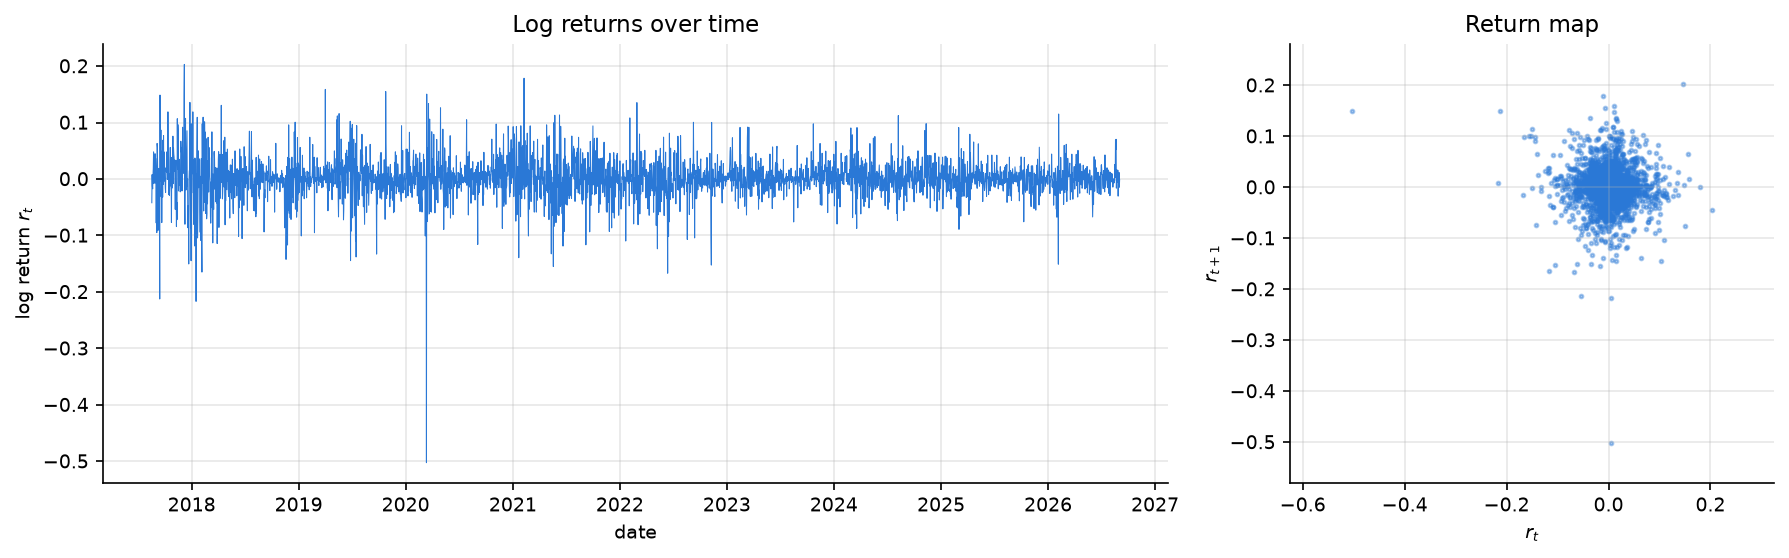
\includegraphics[width=\textwidth,height=0.55\textheight,keepaspectratio]{01_returns_and_return_map.png}
    \begin{itemize}\small
        \item Bursts of large moves (2020 crash, 2021 to 2022) but no visible cycle.
        \item Return map $r_t$ vs $r_{t+1}$ is a round cloud: no thin curve of a deterministic map.
    \end{itemize}
\end{frame}

\begin{frame}{6. Phase Space and Recurrence}
    \begin{columns}[T]
        \begin{column}{0.58\textwidth}
            \centering
            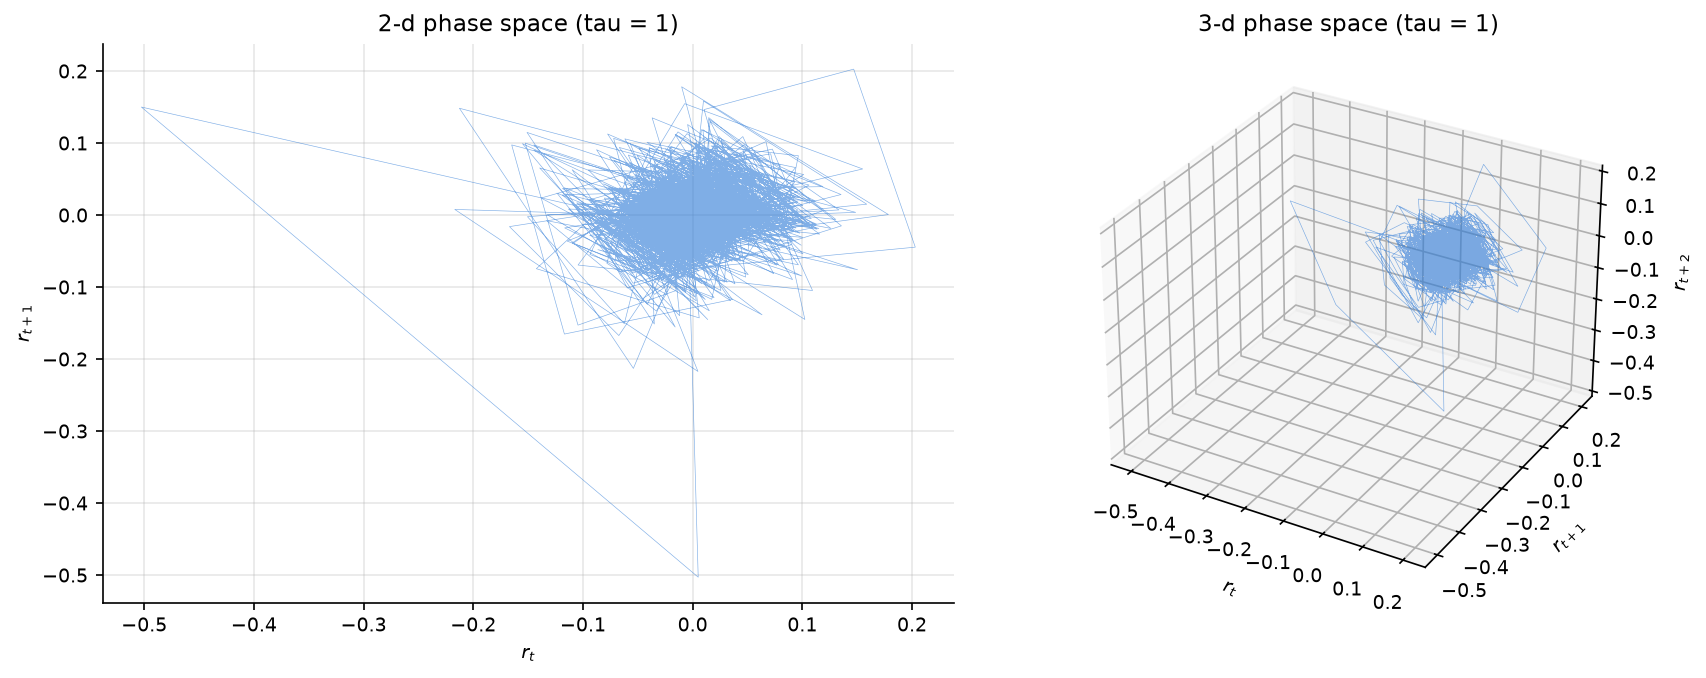
\includegraphics[width=\textwidth]{04_phase_space.png}
        \end{column}
        \begin{column}{0.4\textwidth}
            \centering
            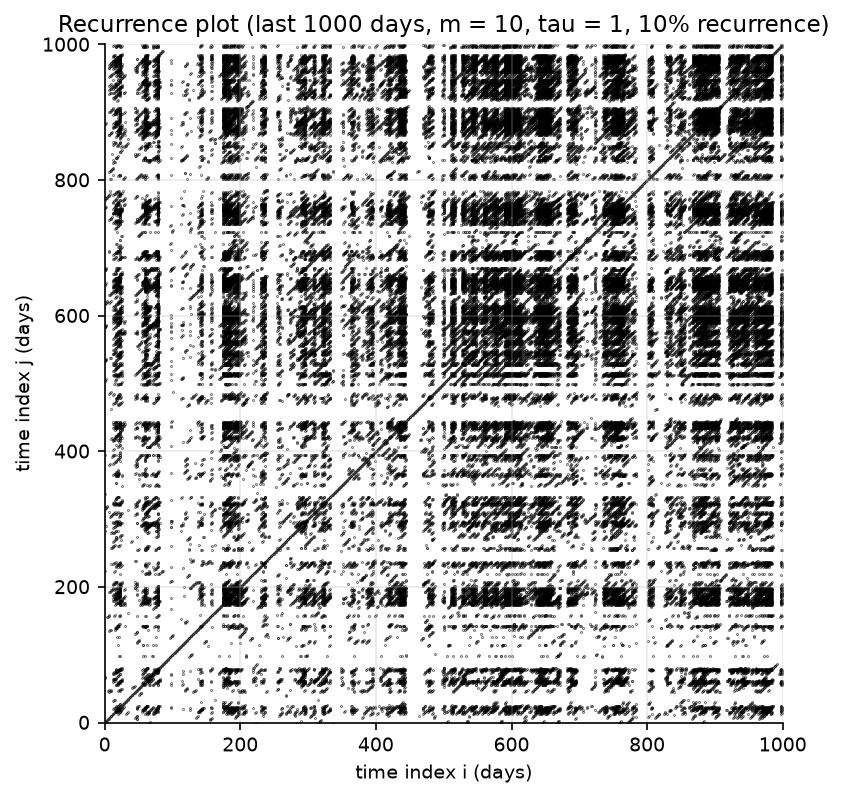
\includegraphics[width=0.85\textwidth]{05_recurrence_plot.png}
        \end{column}
    \end{columns}
    \vspace{4pt}
    \begin{itemize}\small
        \item 2-d and 3-d reconstructions ($\tau=1$): a dense ball, no folded structure.
        \item Recurrence plot: square \textbf{blocks} (calm and turbulent periods), not long diagonal lines.
    \end{itemize}
\end{frame}

\begin{frame}{7. Delay and Dimension}
    \begin{columns}[T]
        \begin{column}{0.48\textwidth}
            \centering
            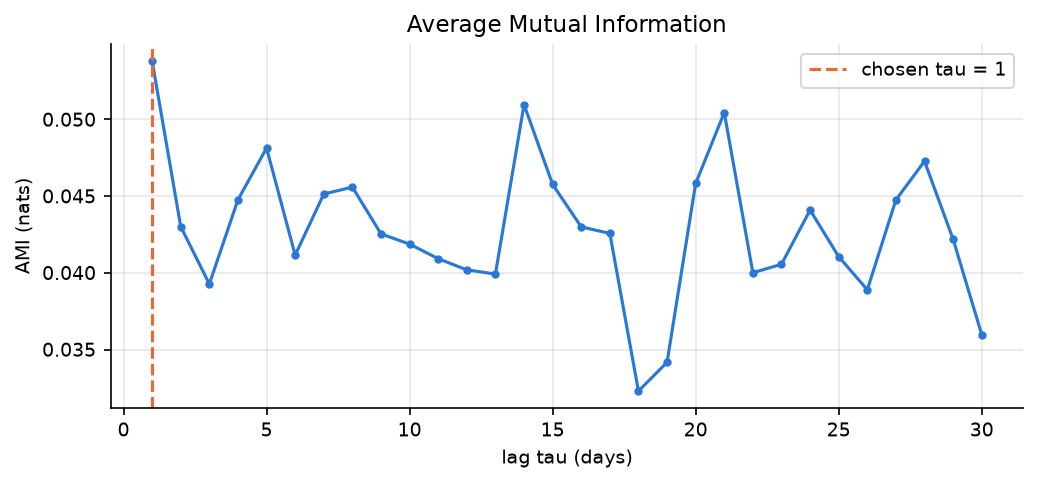
\includegraphics[width=\textwidth]{02_ami.png}\\
            \small AMI is low at all lags; $\tau = 1$.
        \end{column}
        \begin{column}{0.48\textwidth}
            \centering
            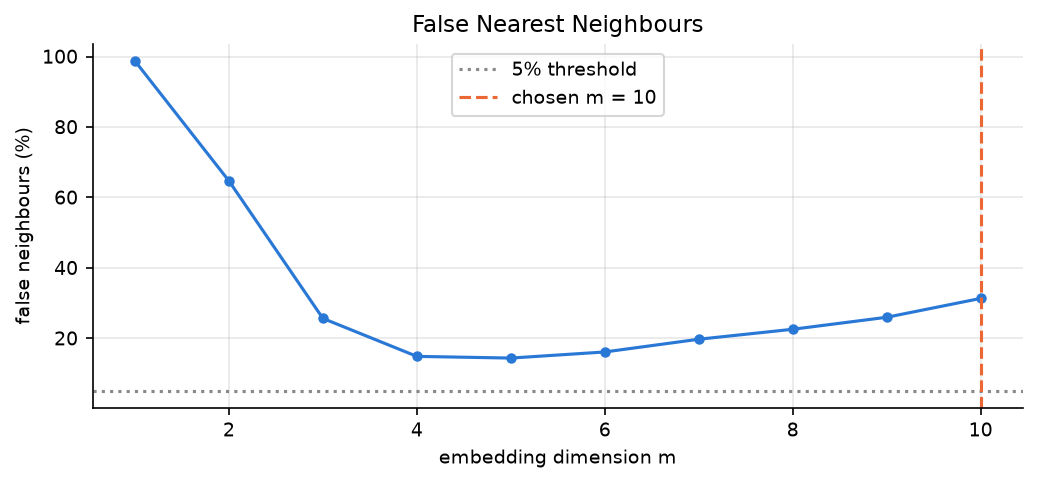
\includegraphics[width=\textwidth]{03_fnn.png}\\
            \small False neighbours bottom out at 14\% ($m=5$) and rise again; the 5\% threshold is never reached.
        \end{column}
    \end{columns}
    \takeaway{The dynamics never ``unfold'' in up to 10 dimensions: the signature of a stochastic series.}
\end{frame}

\begin{frame}{8. Lyapunov Exponent and Correlation Dimension}
    \begin{columns}[T]
        \begin{column}{0.4\textwidth}
            \centering
            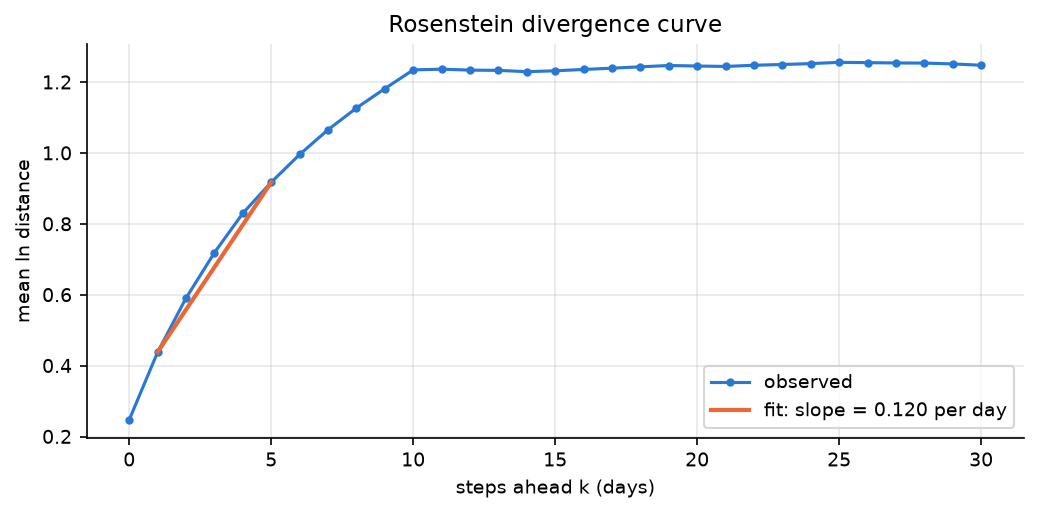
\includegraphics[width=\textwidth]{06_lyapunov.png}
        \end{column}
        \begin{column}{0.58\textwidth}
            \centering
            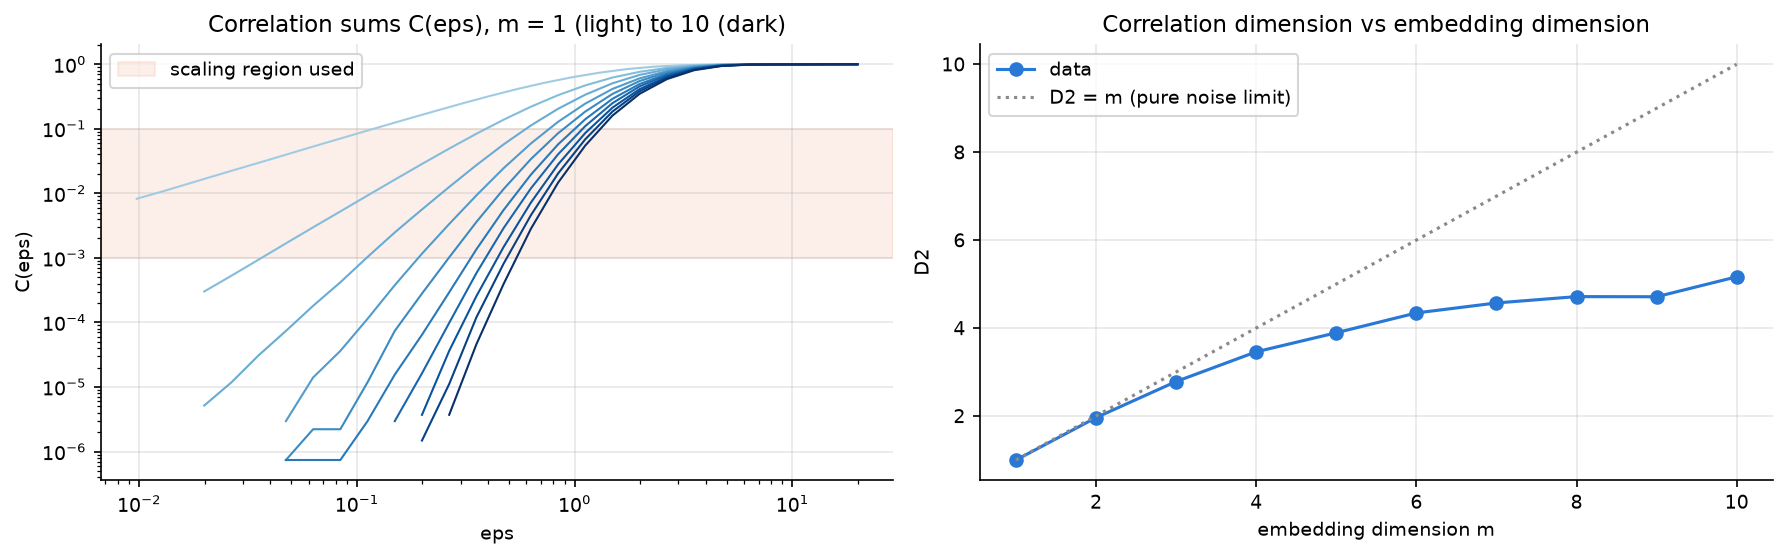
\includegraphics[width=\textwidth]{07_correlation_dimension.png}
        \end{column}
    \end{columns}
    \vspace{4pt}
    \begin{itemize}\small
        \item $\lambda_1 = 0.120$ per day, $R^2=0.99$: positive, but surrogates give 0.11 to 0.14.
        \item $D_2$ levels off near 4.5: far too high for a simple attractor; noise of this length levels off at the same height.
        \item 0--1 test: $K = 0.997$ (irregular, chaos or noise).
    \end{itemize}
\end{frame}

\begin{frame}{9. Surrogate Test and Classification of Returns}
    \centering
    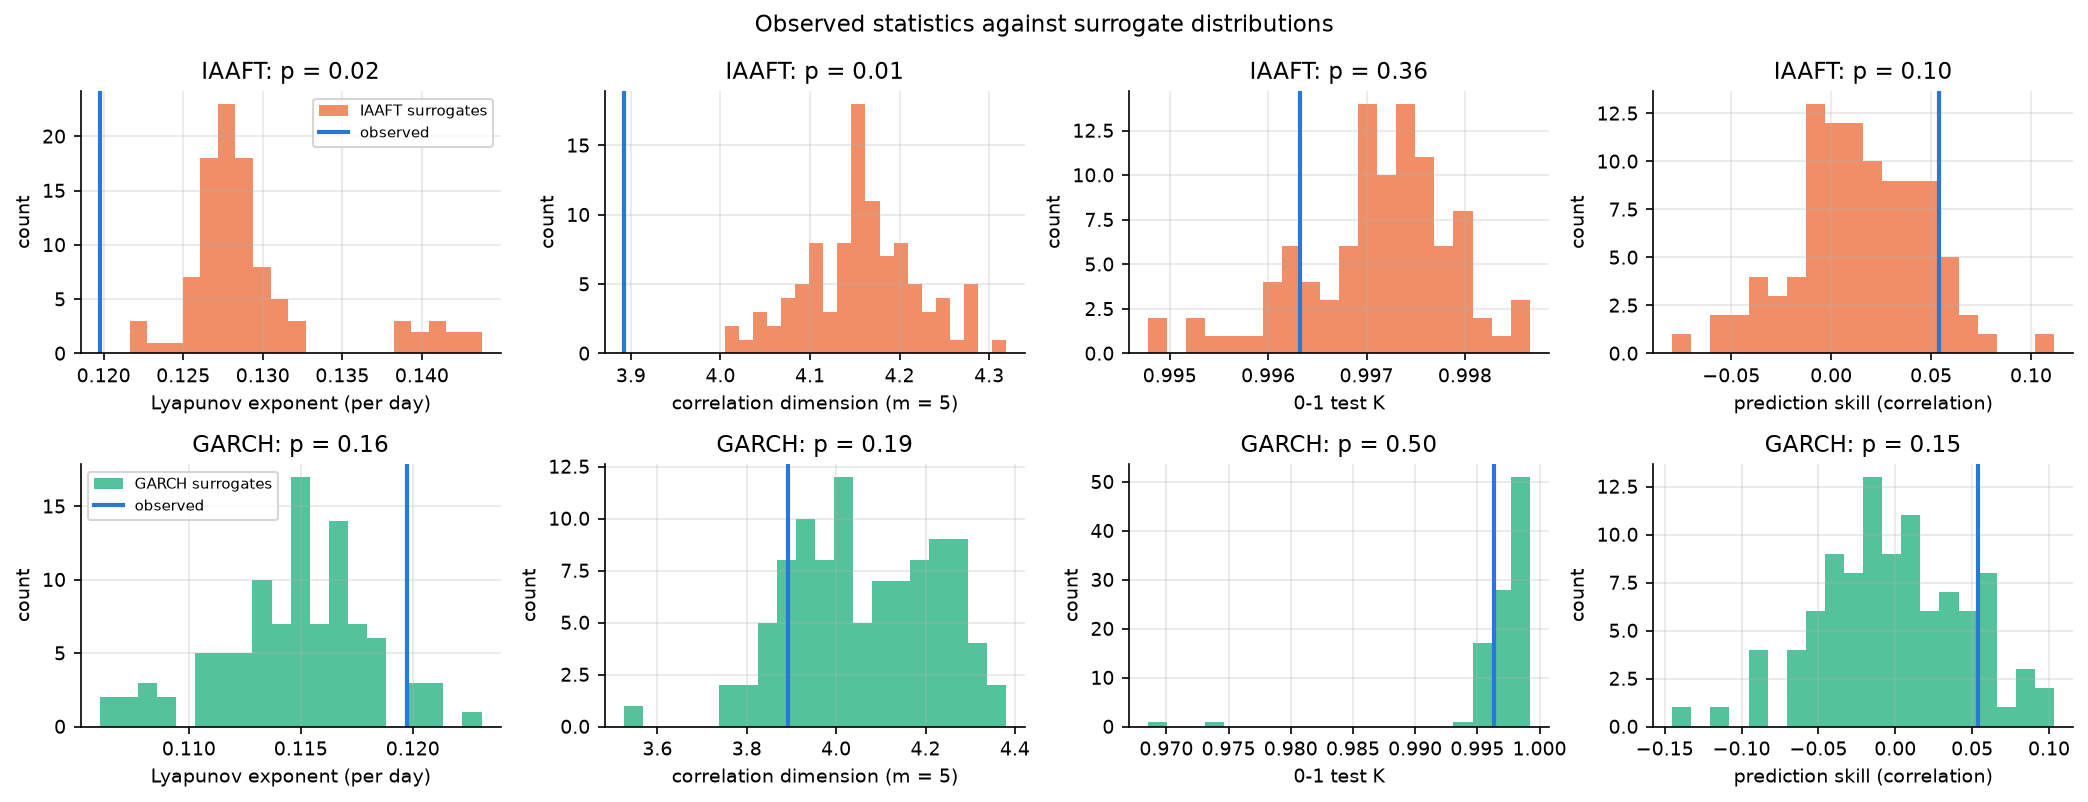
\includegraphics[width=0.92\textwidth,height=0.48\textheight,keepaspectratio]{09_surrogate_test.png}\\[2pt]
    \footnotesize
    \begin{tabular}{lcccc}
        \toprule
        & Lyapunov & $D_2$ ($m=5$) & 0--1 $K$ & prediction skill \\
        \midrule
        $p$ vs IAAFT & 0.02 & 0.01 & 0.36 & 0.10 \\
        $p$ vs GARCH & 0.16 & 0.19 & 0.50 & 0.15 \\
        \bottomrule
    \end{tabular}
    \takeaway{Returns differ from IAAFT (nonlinear) but not from GARCH. Classification: \textbf{Random/Stochastic}.}
\end{frame}

% ==============================================================================
\section{Part B: Returns vs Volatility}

\begin{frame}{10. The Four Series and Their Memory}
    \begin{columns}[T]
        \begin{column}{0.5\textwidth}
            \centering
            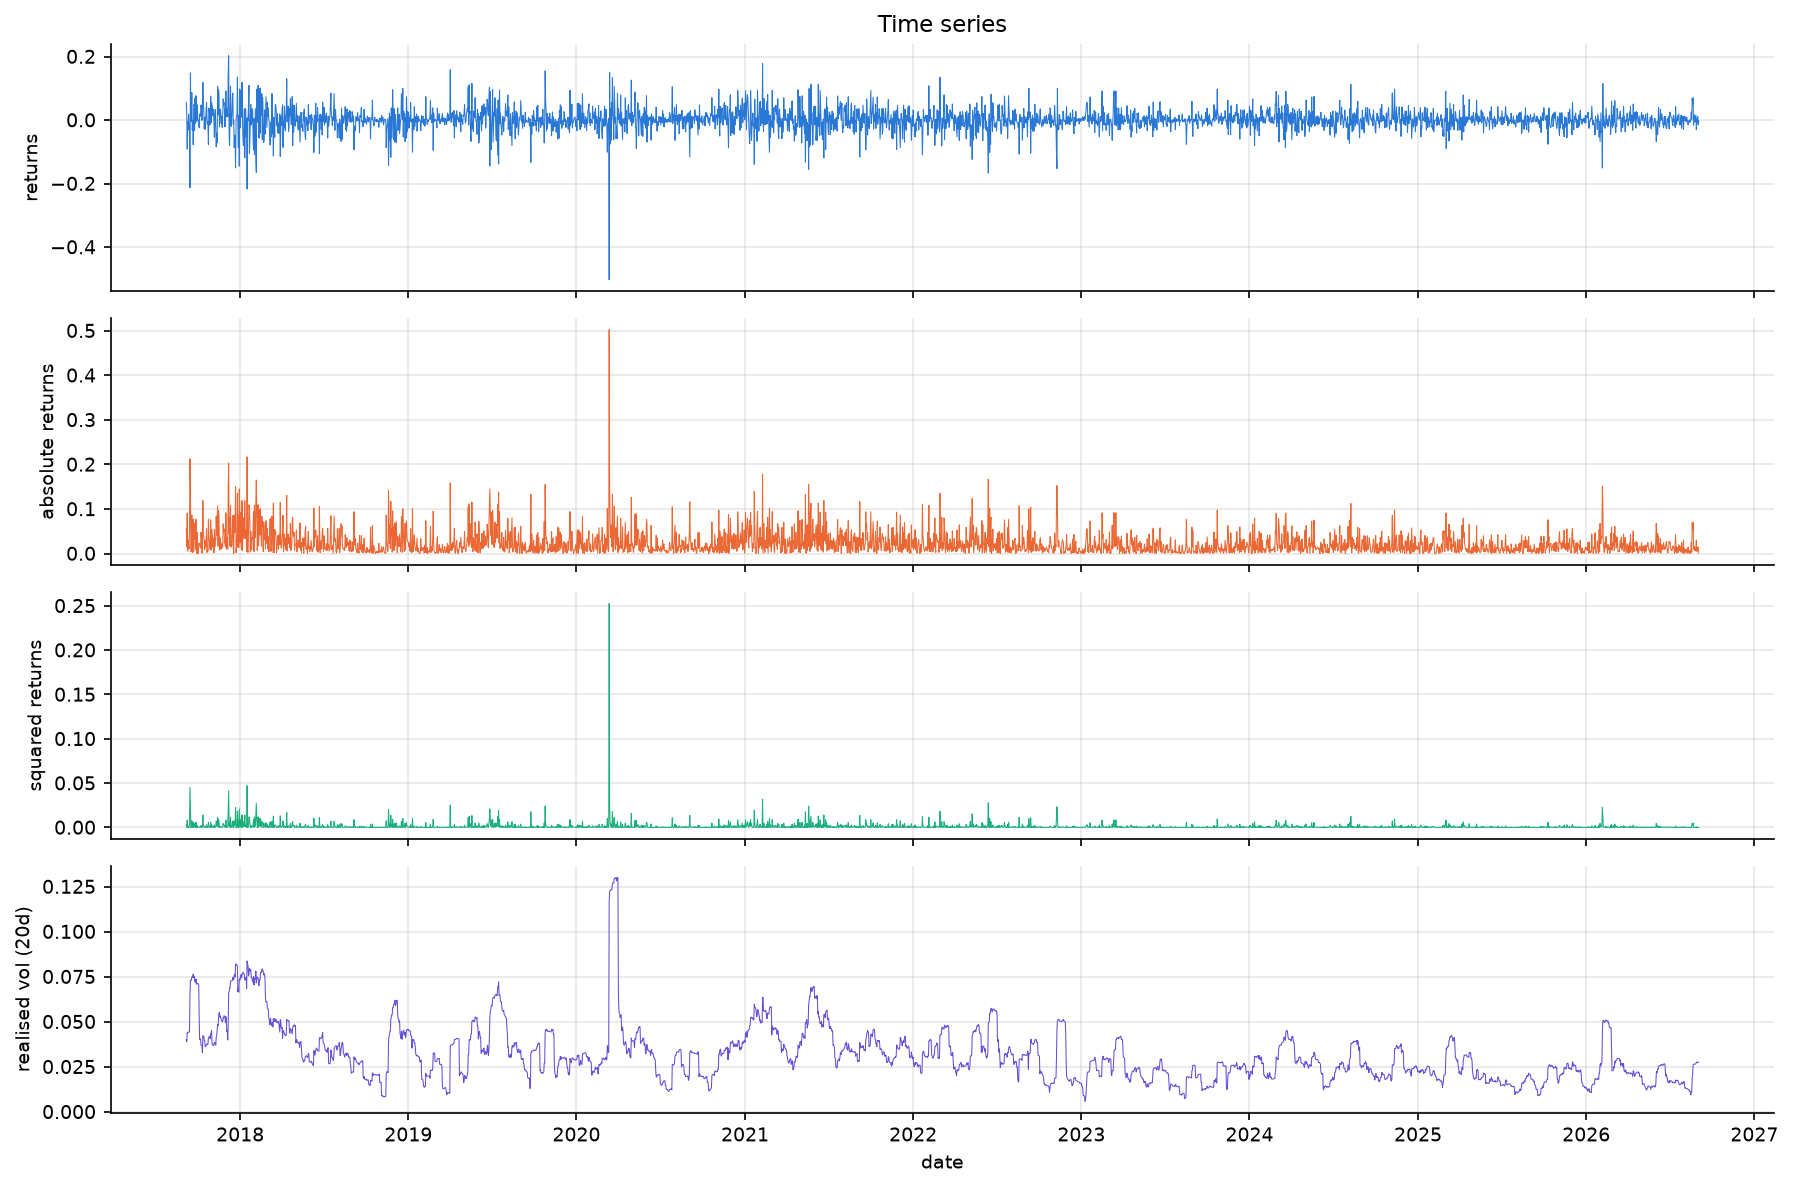
\includegraphics[width=\textwidth,height=0.62\textheight,keepaspectratio]{01_time_series.png}
        \end{column}
        \begin{column}{0.48\textwidth}
            \small
            \begin{itemize}
                \item Returns: autocorrelation close to zero (largest $-0.05$ at lag 1).
                \item Absolute and squared returns: small but very \textbf{persistent} autocorrelation (volatility clustering).
                \item Realised volatility: strong autocorrelation, partly built in by the overlapping 20-day window.
                \item KPSS rejects stationarity for all three volatility series.
            \end{itemize}
        \end{column}
    \end{columns}
    \vspace{2pt}
    \centering
    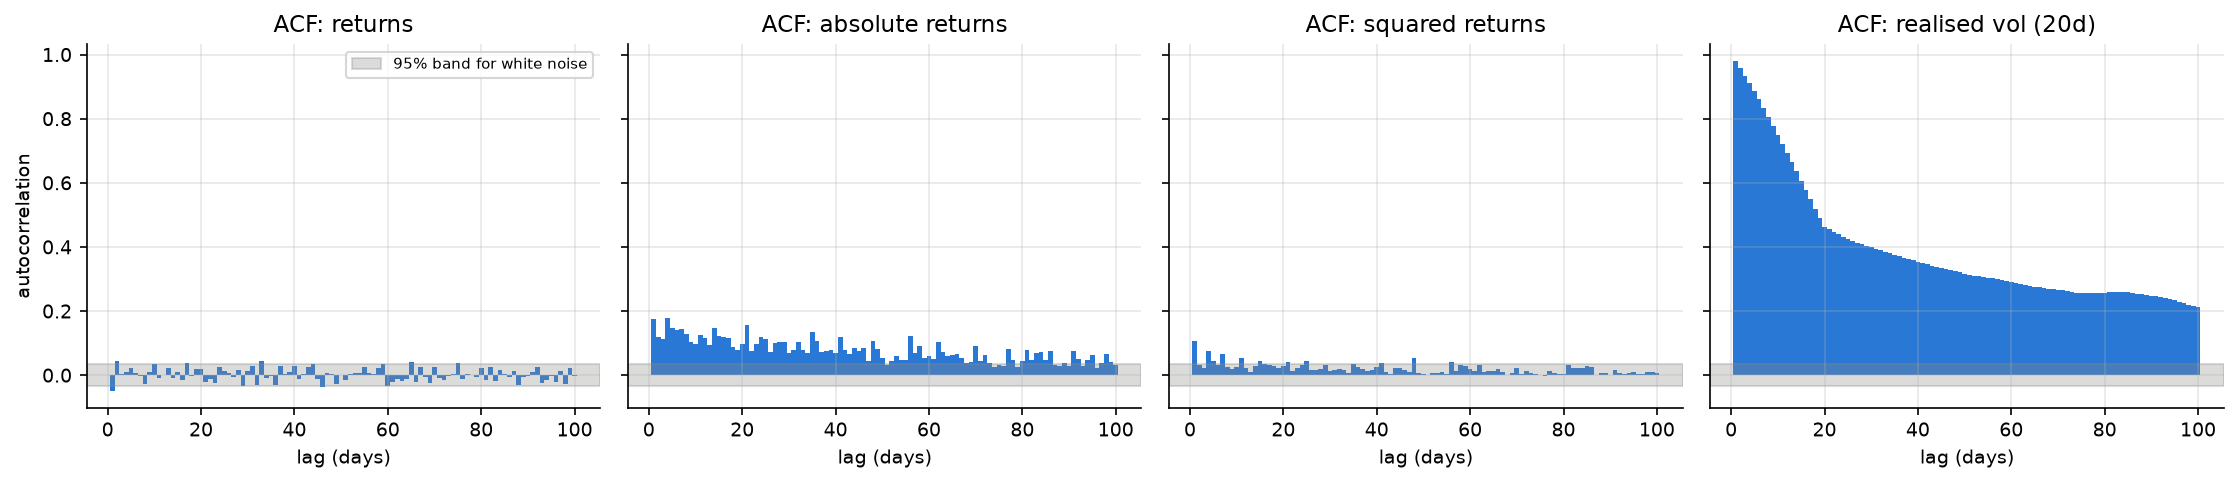
\includegraphics[width=\textwidth,height=0.2\textheight,keepaspectratio]{02_acf.png}
\end{frame}

\begin{frame}{11. Lag Plots and Recurrence Plots}
    \centering
    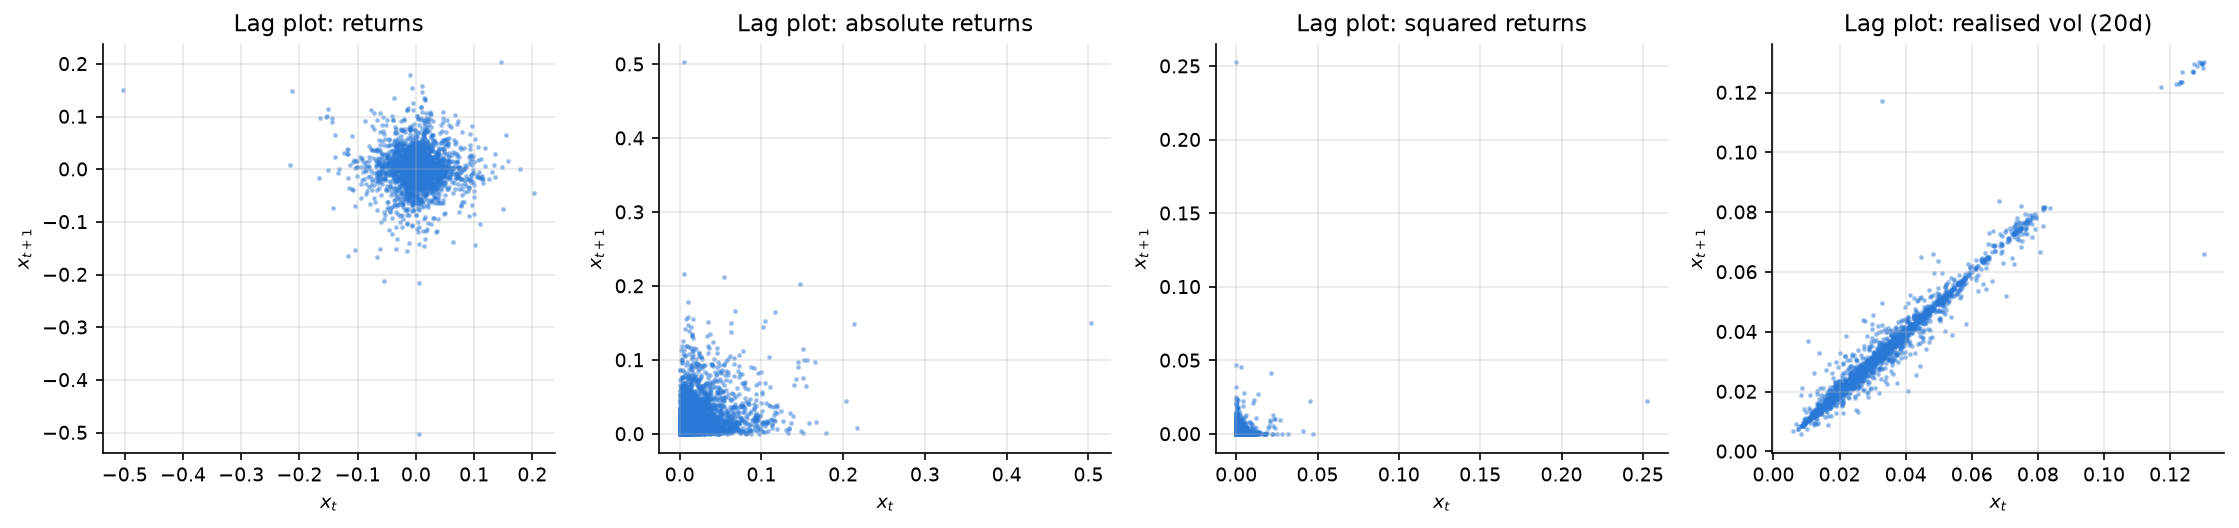
\includegraphics[width=\textwidth,height=0.3\textheight,keepaspectratio]{03_lag_plots.png}\\[2pt]
    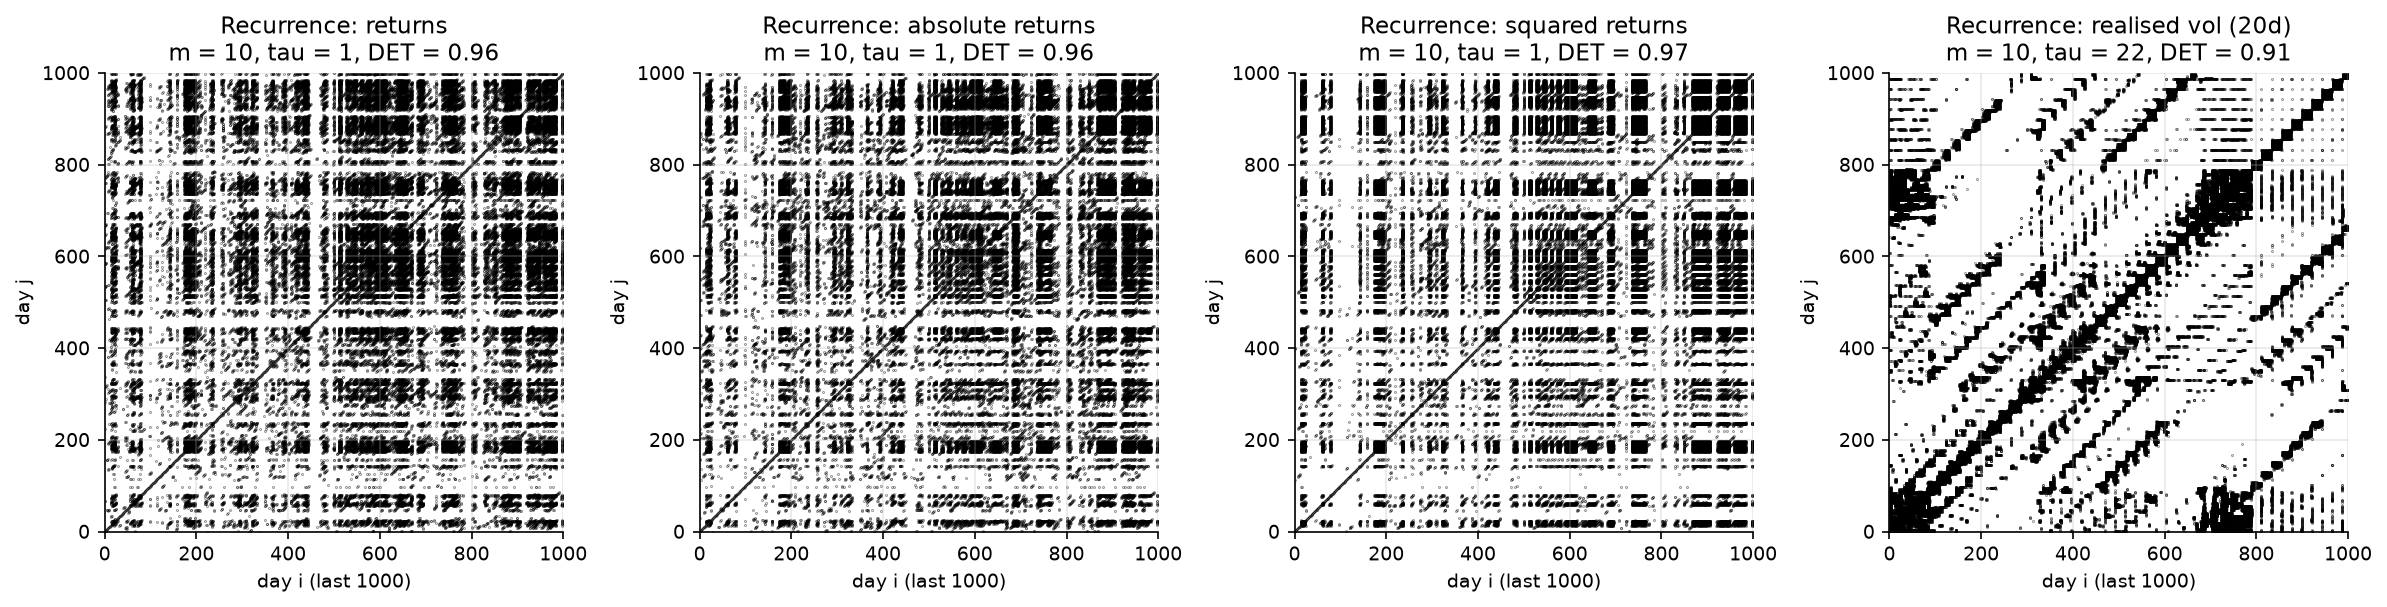
\includegraphics[width=\textwidth,height=0.3\textheight,keepaspectratio]{06_recurrence.png}
    \begin{itemize}\small
        \item Volatility lag plots are tilted wedges (persistence), not thin curves.
        \item Recurrence: blocks for daily series; diagonal bands for realised volatility caused by the 20-day smoothing.
    \end{itemize}
\end{frame}

\begin{frame}{12. Chaos Diagnostics for All Four Series}
    \centering
    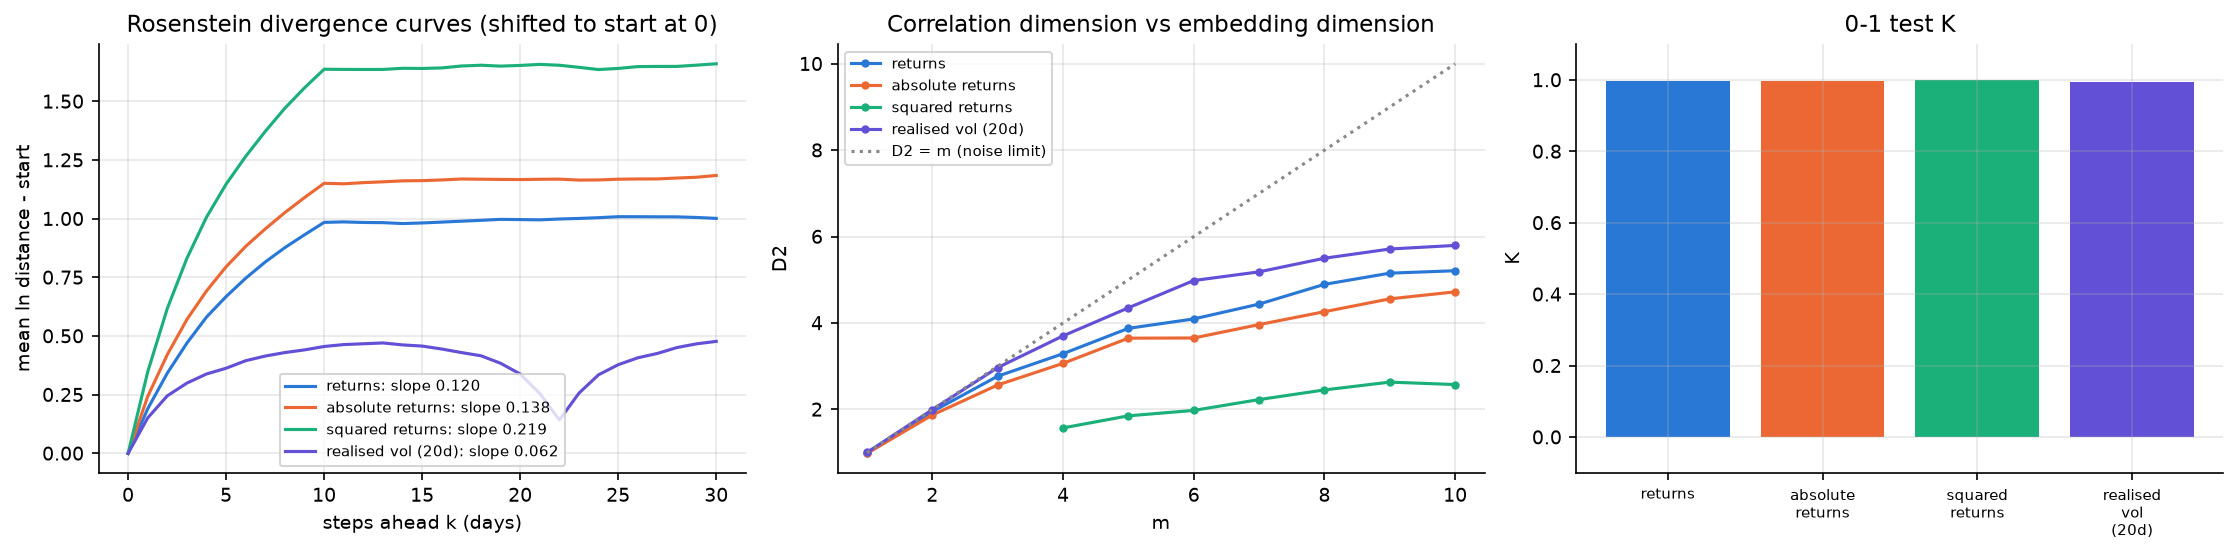
\includegraphics[width=\textwidth,height=0.45\textheight,keepaspectratio]{08_chaos_diagnostics.png}\\[2pt]
    \footnotesize
    \begin{tabular}{lcccc}
        \toprule
        & returns & $\lvert r\rvert$ & $r^2$ & RV (20d) \\
        \midrule
        $\tau$ / $m$ (FNN 5\% reached?) & 1 / 10 (no) & 1 / 10 (no) & 1 / 10 (no) & 22 / 10 (no) \\
        Lyapunov (per day) & 0.120 & 0.138 & 0.219 & 0.062 \\
        $D_2$ (levels off at) & 4.1 & 3.8 & 2.6 & 5.2 \\
        0--1 test $K$ & 1.00 & 1.00 & 1.00 & 0.99 \\
        \bottomrule
    \end{tabular}
\end{frame}

\begin{frame}{13. Realised Volatility Against Its Surrogates}
    \centering
    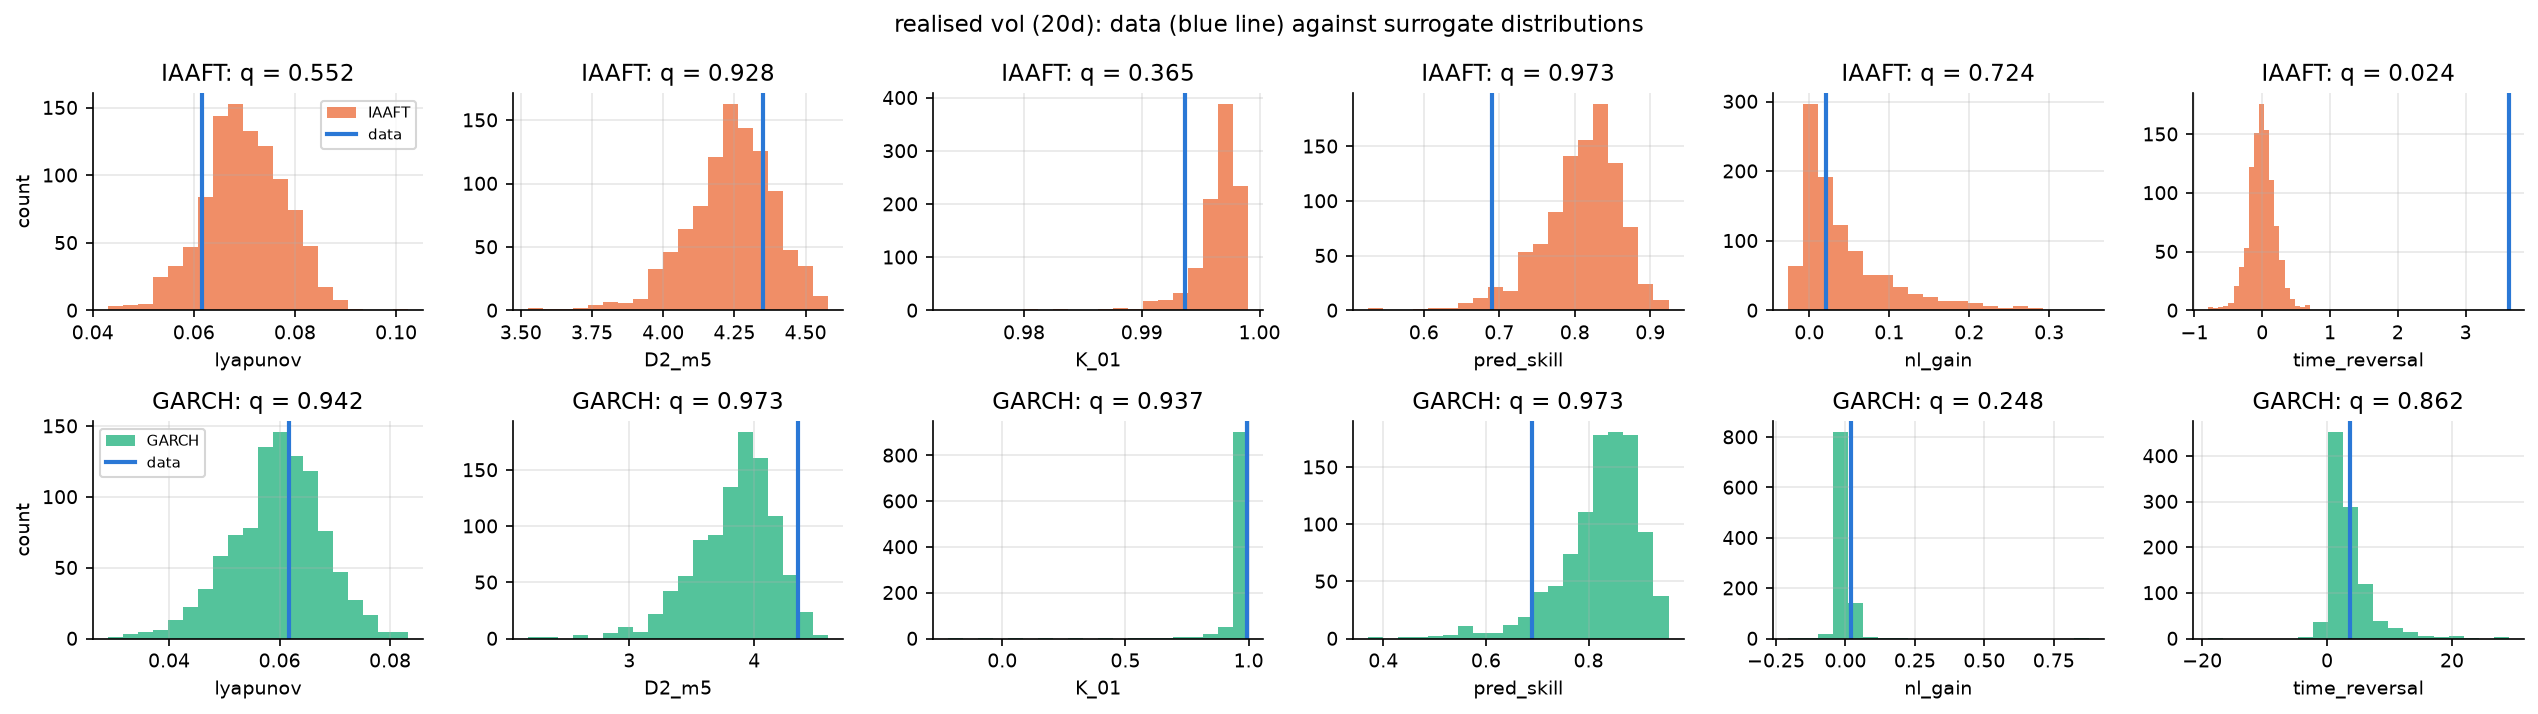
\includegraphics[width=\textwidth,height=0.55\textheight,keepaspectratio]{09_surrogates_realised_vol_20d.png}
    \begin{itemize}\small
        \item Top (IAAFT): time-reversal asymmetry is far outside the surrogates ($z = 18.6$, $q = 0.024$).
        \item Bottom (GARCH): the same asymmetry is right in the middle ($z = 0.01$). Every other statistic matches too.
    \end{itemize}
\end{frame}

\begin{frame}{14. Comparison Table}
    \centering
    \footnotesize
    \begin{tabular}{lcccc}
        \toprule
        & returns & $\lvert r\rvert$ & $r^2$ & RV (20d) \\
        \midrule
        Differs from IAAFT (FDR) & Lyapunov, $D_2$, & Lyapunov, & S-map gain & asymmetry \\
        & asymmetry & asymmetry & & \\
        Differs from GARCH (FDR) & none & none & none & none \\
        Nonlinear & \yes & \yes & \yes & \yes \\
        Beyond GARCH & \no & \no & \no & \no \\
        \midrule
        Time-reversal $z$ vs IAAFT & 5.4 & 2.9 & 0.9 & 18.6 \\
        S-map gain (z vs IAAFT) & 0.005 (1.6) & 0.006 (0.3) & 0.146 (1.9) & 0.021 ($-0.4$) \\
        \midrule
        \textbf{Classification} & \textbf{Random/Stoch.} & \textbf{Random/Stoch.} & \textbf{Random/Stoch.} & \textbf{Random/Stoch.} \\
        \bottomrule
    \end{tabular}
    \takeaway{All four series are nonlinear, none goes beyond GARCH, none meets the rule for potential chaos.}
\end{frame}

\begin{frame}{15. Is Volatility More Nonlinear Than Returns?}
    \centering
    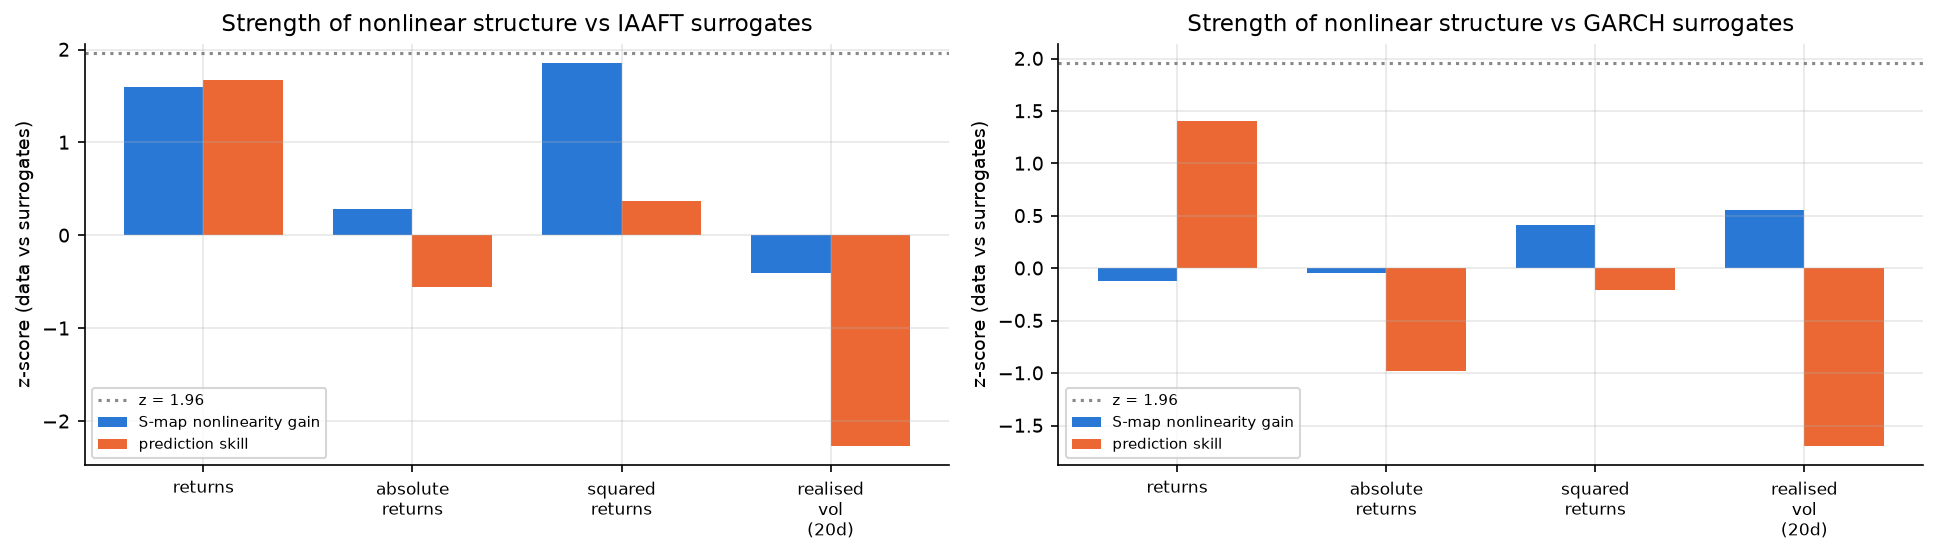
\includegraphics[width=\textwidth,height=0.45\textheight,keepaspectratio]{10_nonlinearity_strength.png}
    \begin{itemize}\small
        \item \textbf{Asymmetry:} yes. Realised volatility rises fast and decays slowly ($z = 18.6$ vs 5.4 for returns).
        \item \textbf{Predictability:} no. Nonlinear forecasts of volatility are not better than for surrogates; against GARCH all $z$-scores are small.
    \end{itemize}
\end{frame}

\begin{frame}{16. Non-Stationarity: Split-Sample Check}
    \centering
    \small
    Full test repeated on each half (GARCH refitted, 499 surrogates, FDR within each half).

    \vspace{6pt}
    \footnotesize
    \begin{tabular}{lcccc}
        \toprule
        Differs from IAAFT & returns & $\lvert r\rvert$ & $r^2$ & RV (20d) \\
        \midrule
        Full sample & Lyap., $D_2$, asym. & Lyap., asym. & S-map gain & asymmetry \\
        2017-09 to 2022-02 & $D_2$ & asymmetry & $D_2$ & asymmetry \\
        2022-02 to 2026-09 & none & none & none & none \\
        \midrule
        Differs from GARCH (any period) & none & none & none & none \\
        \bottomrule
    \end{tabular}
    \takeaway{The nonlinearity comes from the turbulent 2017 to 2022 regime and disappears after 2022: a sign of volatility regimes, not of a stable deterministic attractor.}
\end{frame}

% ==============================================================================
\section{Conclusions}

\begin{frame}{17. Research Interpretation}
    \small
    \begin{enumerate}
        \item \textbf{Volatility contains nonlinear dependence.} So do returns. The strongest signature is the time asymmetry of realised volatility.
        \item \textbf{GARCH explains it completely.} No statistic of any series differs from GARCH(1,1)-$t$ surrogates (smallest $q = 0.22$).
        \item \textbf{No convincing evidence of deterministic chaos.} FNN never converges, $D_2$ levels off only at 2.6 to 5.2 like noise, $\lambda_1>0$ and $K\approx1$ also hold for the surrogates.
        \item \textbf{Classification:} returns, absolute returns, squared returns and realised volatility are all \textbf{Random/Stochastic}: nonlinear, but stochastic.
        \item \textbf{Time variation:} the nonlinear structure is concentrated in 2017 to 2022.
    \end{enumerate}
    \takeaway{BTC behaves like a stochastic volatility process. Nonlinearity is real; chaos is not supported.}
\end{frame}

\begin{frame}{18. Limits and Next Steps}
    \begin{columns}[T]
        \begin{column}{0.48\textwidth}
            \begin{alertblock}{Limits}
                \small
                \begin{itemize}
                    \item About 3300 daily points: enough for low-dimensional chaos, not for high-dimensional chaos.
                    \item Chaos tests lose power quickly with noise.
                    \item Only one asset and one frequency (daily).
                \end{itemize}
            \end{alertblock}
        \end{column}
        \begin{column}{0.48\textwidth}
            \begin{block}{Next steps}
                \small
                \begin{enumerate}
                    \item Test realised volatility against richer stochastic nulls: asymmetric GARCH (GJR, EGARCH), long memory (HAR, FIGARCH), regime switching.
                    \item Repeat with intraday realised volatility.
                    \item Extend to other cryptocurrencies and Nifty 50 stocks.
                \end{enumerate}
            \end{block}
        \end{column}
    \end{columns}
\end{frame}

\begin{frame}
    \centering
    \vspace{2cm}
    {\Large \textbf{Thank you}}\\[10pt]
    Questions and suggestions welcome.
\end{frame}

\end{document}
